%%%%%%%%%%%%%%%%%%%%%%%
% Comp 160, Fall 2019
% Homework 1
% Author: Vladimir Hugec
%%%%%%%%%%%%%%%%%%%%%%%

% This portion of the LaTeX document are configuration 
% You can see it as all the #includes in C++
\documentclass[12pt]{article}

\usepackage{epsfig}
\usepackage{amsmath}
\usepackage{amsthm}
\usepackage{listings}
\usepackage{graphicx}
\usepackage{tikz}

\newtheorem{lemma}{Lemma}
\newtheorem{theorem}{Theorem}

\usepackage{titlesec}
\titleformat{\section}
{\normalfont\Large\bfseries}{Question~\thesection:}{1em}{}

\newlength{\toppush}
\setlength{\toppush}{2\headheight}
\addtolength{\toppush}{\headsep}

\def\subjnum{Comp 170}
\def\subjname{Computation Theory}

\def\doheading#1#2#3{\vfill\eject\vspace*{-\toppush}%
  \vbox{\hbox to\textwidth{{\bf} \subjnum: \subjname \hfil Vladimir Hugec}%
    \hbox to\textwidth{{\bf} Tufts University, Fall 2019 \hfil#3\strut}%
    \hrule}}


\newcommand{\htitle}[1]{\vspace*{1.25ex plus 1ex minus 0ex}%
\begin{center}
{\large\bf #1}
\end{center}} 


%%%%%%%%%%%%%%%%%%%%%%%%%%%%%%%%%%%%%%%%%%%%%%%%%%%%%%%%%%%%%%%%%%%
% BEGIN DOCUMENT
%%%%%%%%%%%%%%%%%%%%%%%%%%%%%%%%%%%%%%%%%%%%%%%%%%%%%%%%%%%%%%%%%%%
\begin{document}
\doheading{2}{title}{Homework 2}

\section{NFA to DFA}

The RegEx for this NFA is: x*y\{1\}x*z*

The NFA has 4 states: a, b, c, d. Therefore the corresponding DFA has the state set:
\begin{center}
\{\O, \{a\}, \{b\}, \{c\}, \{d\}, \{a,b\}, \{a, c\}, \{a, d\}, \{b, c\}, \{b, d\}, \{c, d\}, \newline \{a, b, c\}, \{a, c, d\}, \{b, c, d\}, \{a, b, c, d\}\}
\end{center}

The accept states for the DFA are: 
\begin{center}
\{\{c\}, \{a, c\}, \{b, c\}, \{c, d\}, \{a, b, c\}, \{a, c, d\}, \{a, b, c, d\}\}
\end{center}

$\newline \epsilon$-closure(a) = \{a\}
$\newline \epsilon$-closure(b) = \{b,c,d\}
$\newline \epsilon$-closure(c) = \{c\}
$\newline \epsilon$-closure(d) = \{c,d\}

$\newline$
Transitions
 \begin{tabular}{||c|c|c|c||} 
 \hline
State & x & y & z \\ [0.5ex] 
 \hline\hline
 \{a\} & \{a\} & \{b,c\} & \O \\ 
 \hline
 \{b,c,d\} & \{c,d\} & \O & \O \\
 \hline
 \{c\} & \O & \O & \{c\} \\
 \hline
 \{c,d\} & \{c,d\} & \O & \{c\} \\
 \hline
\end{tabular}

$\newline$
Turning all of this into a graphical representation of the corresponding DFA we get:

\begin{center}
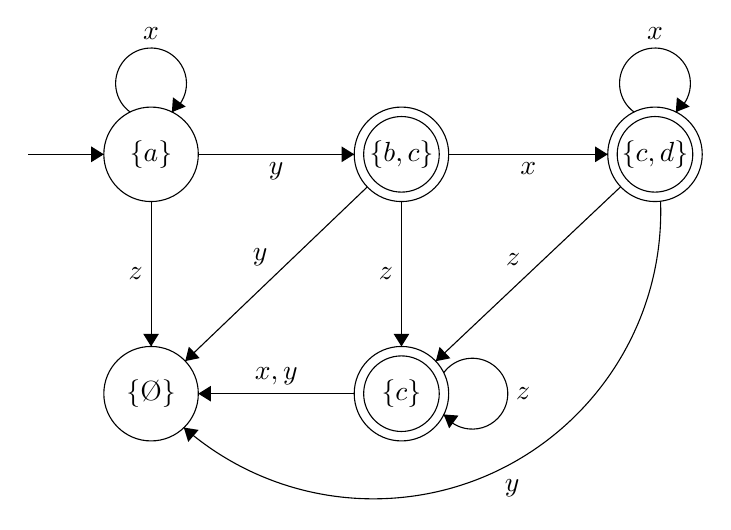
\begin{tikzpicture}[scale=0.2]
\tikzstyle{every node}+=[inner sep=0pt]
\draw [black] (20.2,-15.3) circle (3);
\draw (20.2,-15.3) node {$\{a\}$};
\draw [black] (36.1,-15.3) circle (3);
\draw (36.1,-15.3) node {$\{b,c\}$};
\draw [black] (36.1,-15.3) circle (2.4);
\draw [black] (36.1,-30.5) circle (3);
\draw (36.1,-30.5) node {$\{c\}$};
\draw [black] (36.1,-30.5) circle (2.4);
\draw [black] (20.2,-30.5) circle (3);
\draw (20.2,-30.5) node {$\{\O\}$};
\draw [black] (52.2,-15.3) circle (3);
\draw (52.2,-15.3) node {$\{c,d\}$};
\draw [black] (52.2,-15.3) circle (2.4);
\draw [black] (12.4,-15.3) -- (17.2,-15.3);
\fill [black] (17.2,-15.3) -- (16.4,-14.8) -- (16.4,-15.8);
\draw [black] (23.2,-15.3) -- (33.1,-15.3);
\fill [black] (33.1,-15.3) -- (32.3,-14.8) -- (32.3,-15.8);
\draw (28.15,-15.8) node [below] {$y$};
\draw [black] (18.877,-12.62) arc (234:-54:2.25);
\draw (20.2,-8.05) node [above] {$x$};
\fill [black] (21.52,-12.62) -- (22.4,-12.27) -- (21.59,-11.68);
\draw [black] (36.1,-18.3) -- (36.1,-27.5);
\fill [black] (36.1,-27.5) -- (36.6,-26.7) -- (35.6,-26.7);
\draw (35.6,-22.9) node [left] {$z$};
\draw [black] (20.2,-18.3) -- (20.2,-27.5);
\fill [black] (20.2,-27.5) -- (20.7,-26.7) -- (19.7,-26.7);
\draw (19.7,-22.9) node [left] {$z$};
\draw [black] (39.1,-15.3) -- (49.2,-15.3);
\fill [black] (49.2,-15.3) -- (48.4,-14.8) -- (48.4,-15.8);
\draw (44.15,-15.8) node [below] {$x$};
\draw [black] (33.93,-17.37) -- (22.37,-28.43);
\fill [black] (22.37,-28.43) -- (23.29,-28.24) -- (22.6,-27.51);
\draw (27.13,-22.42) node [above] {$y$};
\draw [black] (38.78,-29.177) arc (144:-144:2.25);
\draw (43.35,-30.5) node [right] {$z$};
\fill [black] (38.78,-31.82) -- (39.13,-32.7) -- (39.72,-31.89);
\draw [black] (33.1,-30.5) -- (23.2,-30.5);
\fill [black] (23.2,-30.5) -- (24,-31) -- (24,-30);
\draw (28.15,-30) node [above] {$x,y$};
\draw [black] (50.877,-12.62) arc (234:-54:2.25);
\draw (52.2,-8.05) node [above] {$x$};
\fill [black] (53.52,-12.62) -- (54.4,-12.27) -- (53.59,-11.68);
\draw [black] (52.552,-18.276) arc (2.04293:-131.22749:18.251);
\fill [black] (22.28,-32.65) -- (22.56,-33.56) -- (23.22,-32.8);
\draw (43.13,-35.92) node [below] {$y$};
\draw [black] (50.02,-17.36) -- (38.28,-28.44);
\fill [black] (38.28,-28.44) -- (39.21,-28.25) -- (38.52,-27.53);
\draw (43.19,-22.42) node [above] {$z$};
\end{tikzpicture}
\end{center}

\pagebreak

\section{RegEx to NFA}

$\newline$
a $\newline$
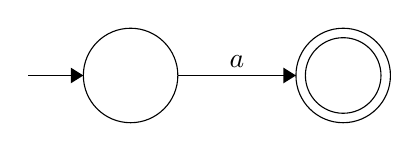
\begin{tikzpicture}[scale=0.2]
\tikzstyle{every node}+=[inner sep=0pt]
\draw [black] (29.3,-20.2) circle (3);
\draw [black] (42.8,-20.2) circle (3);
\draw [black] (42.8,-20.2) circle (2.4);
\draw [black] (32.3,-20.2) -- (39.8,-20.2);
\fill [black] (39.8,-20.2) -- (39,-19.7) -- (39,-20.7);
\draw (36.05,-19.7) node [above] {$a$};
\draw [black] (22.8,-20.2) -- (26.3,-20.2);
\fill [black] (26.3,-20.2) -- (25.5,-19.7) -- (25.5,-20.7);
\end{tikzpicture}

$\newline$
b 
$\newline$
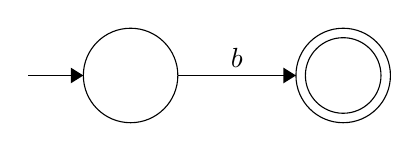
\begin{tikzpicture}[scale=0.2]
\tikzstyle{every node}+=[inner sep=0pt]
\draw [black] (29.3,-20.2) circle (3);
\draw [black] (42.8,-20.2) circle (3);
\draw [black] (42.8,-20.2) circle (2.4);
\draw [black] (32.3,-20.2) -- (39.8,-20.2);
\fill [black] (39.8,-20.2) -- (39,-19.7) -- (39,-20.7);
\draw (36.05,-19.7) node [above] {$b$};
\draw [black] (22.8,-20.2) -- (26.3,-20.2);
\fill [black] (26.3,-20.2) -- (25.5,-19.7) -- (25.5,-20.7);
\end{tikzpicture}

$\newline$
a*
$\newline$
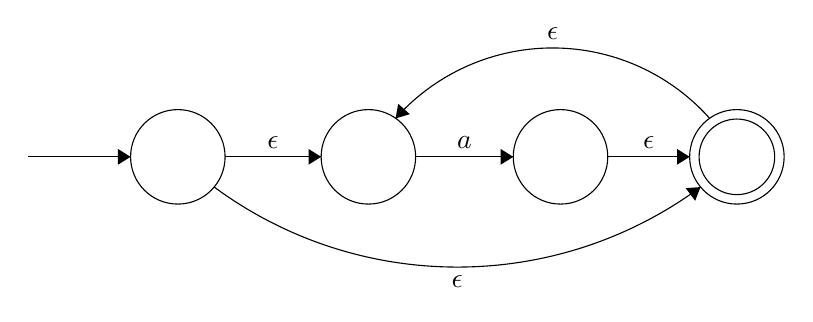
\begin{tikzpicture}[scale=0.2]
\tikzstyle{every node}+=[inner sep=0pt]
\draw [black] (23,-21.7) circle (3);
\draw [black] (35.1,-21.7) circle (3);
\draw [black] (58.5,-21.7) circle (3);
\draw [black] (58.5,-21.7) circle (2.4);
\draw [black] (47.3,-21.7) circle (3);
\draw [black] (13.5,-21.7) -- (20,-21.7);
\fill [black] (20,-21.7) -- (19.2,-21.2) -- (19.2,-22.2);
\draw [black] (26,-21.7) -- (32.1,-21.7);
\fill [black] (32.1,-21.7) -- (31.3,-21.2) -- (31.3,-22.2);
\draw (29.05,-21.2) node [above] {$\epsilon$};
\draw [black] (56.195,-23.617) arc (-53.5626:-126.4374:26.003);
\fill [black] (56.19,-23.62) -- (55.25,-23.69) -- (55.85,-24.49);
\draw (40.75,-29.2) node [below] {$\epsilon$};
\draw [black] (36.829,-19.256) arc (138.29317:41.70683:13.356);
\fill [black] (36.83,-19.26) -- (37.73,-18.99) -- (36.99,-18.33);
\draw (46.8,-14.29) node [above] {$\epsilon$};
\draw [black] (38.1,-21.7) -- (44.3,-21.7);
\fill [black] (44.3,-21.7) -- (43.5,-21.2) -- (43.5,-22.2);
\draw (41.2,-21.2) node [above] {$a$};
\draw [black] (50.3,-21.7) -- (55.5,-21.7);
\fill [black] (55.5,-21.7) -- (54.7,-21.2) -- (54.7,-22.2);
\draw (52.9,-21.2) node [above] {$\epsilon$};
\end{tikzpicture}

$\newline$
b*
$\newline$
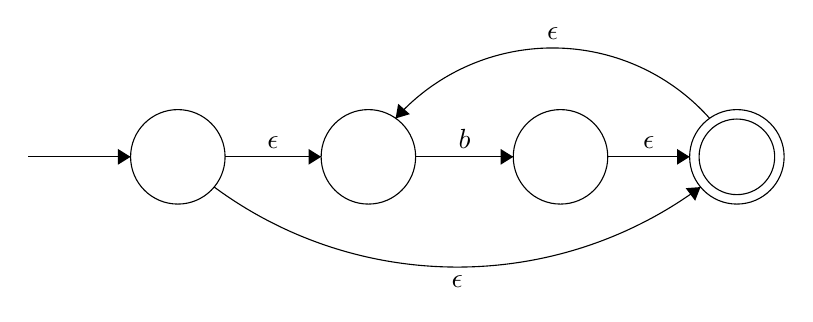
\begin{tikzpicture}[scale=0.2]
\tikzstyle{every node}+=[inner sep=0pt]
\draw [black] (23,-21.7) circle (3);
\draw [black] (35.1,-21.7) circle (3);
\draw [black] (58.5,-21.7) circle (3);
\draw [black] (58.5,-21.7) circle (2.4);
\draw [black] (47.3,-21.7) circle (3);
\draw [black] (13.5,-21.7) -- (20,-21.7);
\fill [black] (20,-21.7) -- (19.2,-21.2) -- (19.2,-22.2);
\draw [black] (26,-21.7) -- (32.1,-21.7);
\fill [black] (32.1,-21.7) -- (31.3,-21.2) -- (31.3,-22.2);
\draw (29.05,-21.2) node [above] {$\epsilon$};
\draw [black] (56.195,-23.617) arc (-53.5626:-126.4374:26.003);
\fill [black] (56.19,-23.62) -- (55.25,-23.69) -- (55.85,-24.49);
\draw (40.75,-29.2) node [below] {$\epsilon$};
\draw [black] (36.829,-19.256) arc (138.29317:41.70683:13.356);
\fill [black] (36.83,-19.26) -- (37.73,-18.99) -- (36.99,-18.33);
\draw (46.8,-14.29) node [above] {$\epsilon$};
\draw [black] (38.1,-21.7) -- (44.3,-21.7);
\fill [black] (44.3,-21.7) -- (43.5,-21.2) -- (43.5,-22.2);
\draw (41.2,-21.2) node [above] {$b$};
\draw [black] (50.3,-21.7) -- (55.5,-21.7);
\fill [black] (55.5,-21.7) -- (54.7,-21.2) -- (54.7,-22.2);
\draw (52.9,-21.2) node [above] {$\epsilon$};
\end{tikzpicture}

\pagebreak
$\newline$
a* U b*
$\newline$
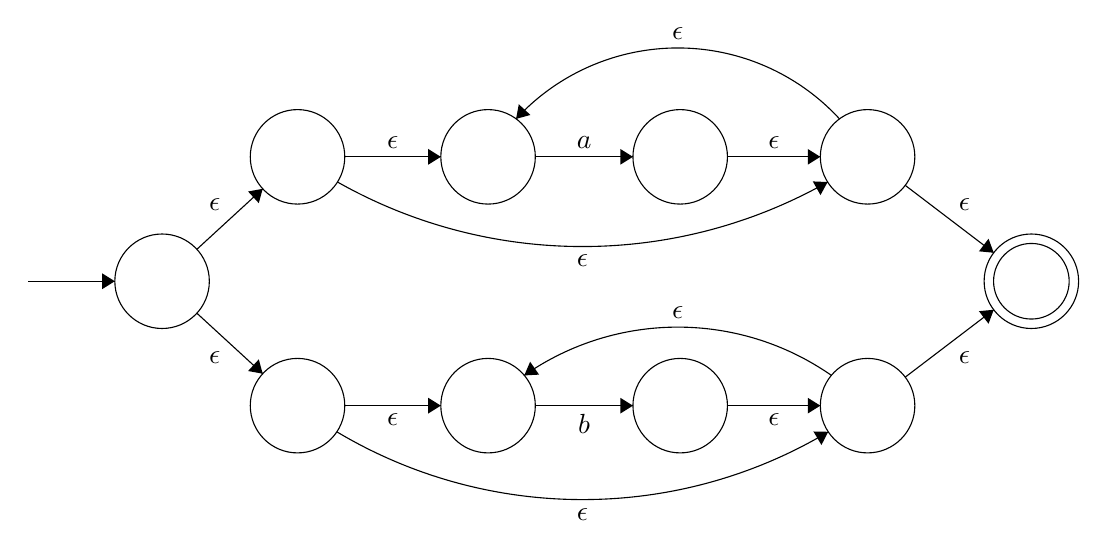
\begin{tikzpicture}[scale=0.2]
\tikzstyle{every node}+=[inner sep=0pt]
\draw [black] (23,-21.7) circle (3);
\draw [black] (35.1,-21.7) circle (3);
\draw [black] (59.2,-21.7) circle (3);
\draw [black] (47.3,-21.7) circle (3);
\draw [black] (23,-37.5) circle (3);
\draw [black] (35.1,-37.5) circle (3);
\draw [black] (47.3,-37.5) circle (3);
\draw [black] (59.2,-37.5) circle (3);
\draw [black] (14.4,-29.6) circle (3);
\draw [black] (69.6,-29.6) circle (3);
\draw [black] (69.6,-29.6) circle (2.4);
\draw [black] (26,-21.7) -- (32.1,-21.7);
\fill [black] (32.1,-21.7) -- (31.3,-21.2) -- (31.3,-22.2);
\draw (29.05,-21.2) node [above] {$\epsilon$};
\draw [black] (56.663,-23.299) arc (-60.49921:-119.50079:31.604);
\fill [black] (56.66,-23.3) -- (55.72,-23.26) -- (56.21,-24.13);
\draw (41.1,-27.9) node [below] {$\epsilon$};
\draw [black] (36.879,-19.292) arc (137.37999:42.62001:13.957);
\fill [black] (36.88,-19.29) -- (37.79,-19.04) -- (37.05,-18.36);
\draw (47.15,-14.29) node [above] {$\epsilon$};
\draw [black] (38.1,-21.7) -- (44.3,-21.7);
\fill [black] (44.3,-21.7) -- (43.5,-21.2) -- (43.5,-22.2);
\draw (41.2,-21.2) node [above] {$a$};
\draw [black] (50.3,-21.7) -- (56.2,-21.7);
\fill [black] (56.2,-21.7) -- (55.4,-21.2) -- (55.4,-22.2);
\draw (53.25,-21.2) node [above] {$\epsilon$};
\draw [black] (26,-37.5) -- (32.1,-37.5);
\fill [black] (32.1,-37.5) -- (31.3,-37) -- (31.3,-38);
\draw (29.05,-38) node [below] {$\epsilon$};
\draw [black] (38.1,-37.5) -- (44.3,-37.5);
\fill [black] (44.3,-37.5) -- (43.5,-37) -- (43.5,-38);
\draw (41.2,-38) node [below] {$b$};
\draw [black] (50.3,-37.5) -- (56.2,-37.5);
\fill [black] (56.2,-37.5) -- (55.4,-37) -- (55.4,-38);
\draw (53.25,-38) node [below] {$\epsilon$};
\draw [black] (5.9,-29.6) -- (11.4,-29.6);
\fill [black] (11.4,-29.6) -- (10.6,-29.1) -- (10.6,-30.1);
\draw [black] (16.61,-27.57) -- (20.79,-23.73);
\fill [black] (20.79,-23.73) -- (19.86,-23.9) -- (20.54,-24.64);
\draw (17.74,-25.16) node [above] {$\epsilon$};
\draw [black] (16.61,-31.63) -- (20.79,-35.47);
\fill [black] (20.79,-35.47) -- (20.54,-34.56) -- (19.86,-35.3);
\draw (17.74,-34.04) node [below] {$\epsilon$};
\draw [black] (56.704,-39.162) arc (-59.16218:-120.83782:30.44);
\fill [black] (56.7,-39.16) -- (55.76,-39.14) -- (56.27,-40);
\draw (41.1,-43.97) node [below] {$\epsilon$};
\draw [black] (37.397,-35.577) arc (124.89171:55.10829:17.049);
\fill [black] (37.4,-35.58) -- (38.34,-35.53) -- (37.77,-34.71);
\draw (47.15,-32.01) node [above] {$\epsilon$};
\draw [black] (61.59,-23.51) -- (67.21,-27.79);
\fill [black] (67.21,-27.79) -- (66.88,-26.9) -- (66.27,-27.7);
\draw (65.35,-25.15) node [above] {$\epsilon$};
\draw [black] (61.59,-35.69) -- (67.21,-31.41);
\fill [black] (67.21,-31.41) -- (66.27,-31.5) -- (66.88,-32.3);
\draw (65.35,-34.05) node [below] {$\epsilon$};
\end{tikzpicture}

$\newline$
(a* U b*) a
$\newline$
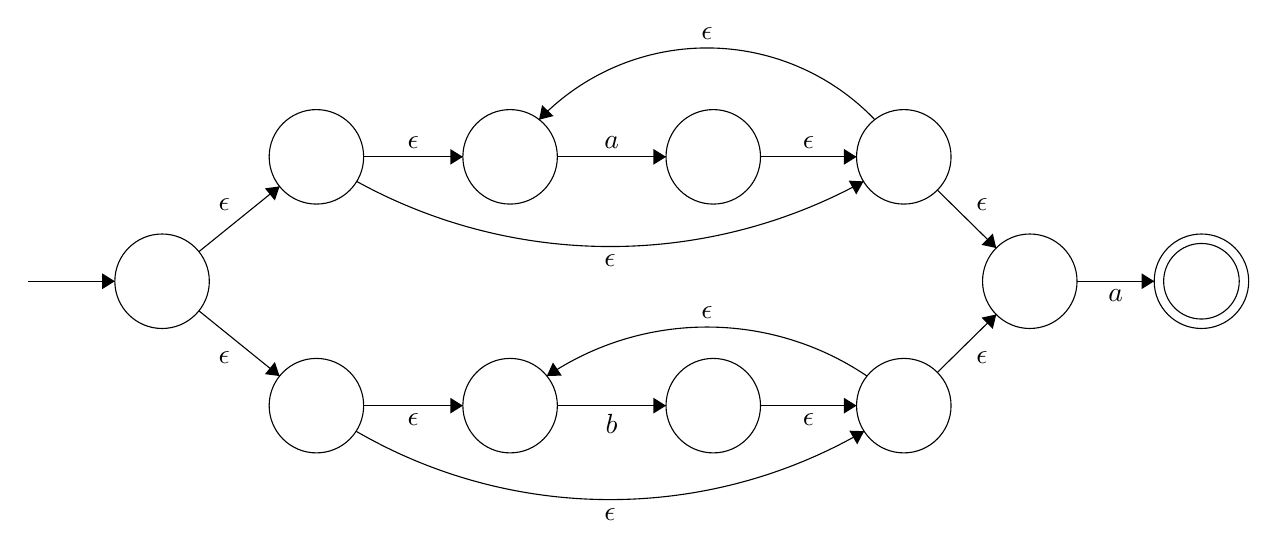
\begin{tikzpicture}[scale=0.2]
\tikzstyle{every node}+=[inner sep=0pt]
\draw [black] (20,-21.7) circle (3);
\draw [black] (32.3,-21.7) circle (3);
\draw [black] (57.3,-21.7) circle (3);
\draw [black] (45.2,-21.7) circle (3);
\draw [black] (20,-37.5) circle (3);
\draw [black] (32.3,-37.5) circle (3);
\draw [black] (45.2,-37.5) circle (3);
\draw [black] (57.3,-37.5) circle (3);
\draw [black] (10.2,-29.6) circle (3);
\draw [black] (65.3,-29.6) circle (3);
\draw [black] (76.2,-29.6) circle (3);
\draw [black] (76.2,-29.6) circle (2.4);
\draw [black] (23,-21.7) -- (29.3,-21.7);
\fill [black] (29.3,-21.7) -- (28.5,-21.2) -- (28.5,-22.2);
\draw (26.15,-21.2) node [above] {$\epsilon$};
\draw [black] (54.74,-23.262) arc (-61.17535:-118.82465:33.373);
\fill [black] (54.74,-23.26) -- (53.8,-23.21) -- (54.28,-24.09);
\draw (38.65,-27.9) node [below] {$\epsilon$};
\draw [black] (34.141,-19.338) arc (136.25163:43.74837:14.756);
\fill [black] (34.14,-19.34) -- (35.06,-19.11) -- (34.33,-18.41);
\draw (44.8,-14.29) node [above] {$\epsilon$};
\draw [black] (35.3,-21.7) -- (42.2,-21.7);
\fill [black] (42.2,-21.7) -- (41.4,-21.2) -- (41.4,-22.2);
\draw (38.75,-21.2) node [above] {$a$};
\draw [black] (48.2,-21.7) -- (54.3,-21.7);
\fill [black] (54.3,-21.7) -- (53.5,-21.2) -- (53.5,-22.2);
\draw (51.25,-21.2) node [above] {$\epsilon$};
\draw [black] (23,-37.5) -- (29.3,-37.5);
\fill [black] (29.3,-37.5) -- (28.5,-37) -- (28.5,-38);
\draw (26.15,-38) node [below] {$\epsilon$};
\draw [black] (35.3,-37.5) -- (42.2,-37.5);
\fill [black] (42.2,-37.5) -- (41.4,-37) -- (41.4,-38);
\draw (38.75,-38) node [below] {$b$};
\draw [black] (48.2,-37.5) -- (54.3,-37.5);
\fill [black] (54.3,-37.5) -- (53.5,-37) -- (53.5,-38);
\draw (51.25,-38) node [below] {$\epsilon$};
\draw [black] (1.7,-29.6) -- (7.2,-29.6);
\fill [black] (7.2,-29.6) -- (6.4,-29.1) -- (6.4,-30.1);
\draw [black] (12.54,-27.72) -- (17.66,-23.58);
\fill [black] (17.66,-23.58) -- (16.73,-23.7) -- (17.36,-24.47);
\draw (14.15,-25.16) node [above] {$\epsilon$};
\draw [black] (12.54,-31.48) -- (17.66,-35.62);
\fill [black] (17.66,-35.62) -- (17.36,-34.73) -- (16.73,-35.5);
\draw (14.15,-34.04) node [below] {$\epsilon$};
\draw [black] (54.779,-39.125) arc (-59.87026:-120.12974:32.133);
\fill [black] (54.78,-39.12) -- (53.84,-39.09) -- (54.34,-39.96);
\draw (38.65,-43.97) node [below] {$\epsilon$};
\draw [black] (34.635,-35.622) arc (124.07449:55.92551:18.143);
\fill [black] (34.63,-35.62) -- (35.58,-35.59) -- (35.02,-34.76);
\draw (44.8,-32.01) node [above] {$\epsilon$};
\draw [black] (59.43,-23.81) -- (63.17,-27.49);
\fill [black] (63.17,-27.49) -- (62.95,-26.57) -- (62.24,-27.29);
\draw (62.27,-25.17) node [above] {$\epsilon$};
\draw [black] (59.43,-35.39) -- (63.17,-31.71);
\fill [black] (63.17,-31.71) -- (62.24,-31.91) -- (62.95,-32.63);
\draw (62.27,-34.03) node [below] {$\epsilon$};
\draw [black] (68.3,-29.6) -- (73.2,-29.6);
\fill [black] (73.2,-29.6) -- (72.4,-29.1) -- (72.4,-30.1);
\draw (70.75,-30.1) node [below] {$a$};
\end{tikzpicture}

\pagebreak

\section{Binary Additive Arithmetic}

The RegEx for the Binary Additive Arithmetic language is: 

\begin{center}
$(0? + 1(1 + 0)$*$) (+|-)  (0? + 1(1 + 0)$*$)$
\end{center}

The corresponding NFA for this language is:

\begin{center}
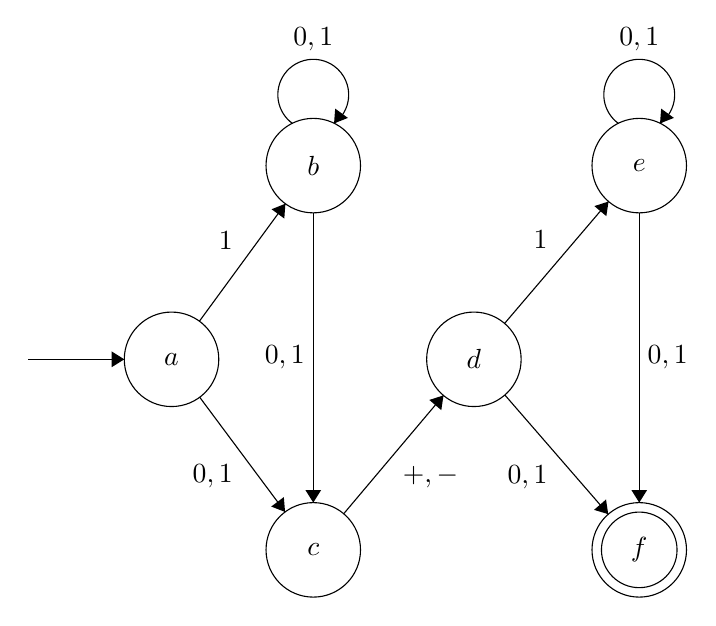
\begin{tikzpicture}[scale=0.2]
\tikzstyle{every node}+=[inner sep=0pt]
\draw [black] (25.1,-30.3) circle (3);
\draw (25.1,-30.3) node {$a$};
\draw [black] (34.1,-18) circle (3);
\draw (34.1,-18) node {$b$};
\draw [black] (34.1,-42.4) circle (3);
\draw (34.1,-42.4) node {$c$};
\draw [black] (44.3,-30.3) circle (3);
\draw (44.3,-30.3) node {$d$};
\draw [black] (54.8,-18) circle (3);
\draw (54.8,-18) node {$e$};
\draw [black] (54.8,-42.4) circle (3);
\draw (54.8,-42.4) node {$f$};
\draw [black] (54.8,-42.4) circle (2.4);
\draw [black] (26.87,-27.88) -- (32.33,-20.42);
\fill [black] (32.33,-20.42) -- (31.45,-20.77) -- (32.26,-21.36);
\draw (29.02,-22.76) node [left] {$1$};
\draw [black] (26.89,-32.71) -- (32.31,-39.99);
\fill [black] (32.31,-39.99) -- (32.23,-39.05) -- (31.43,-39.65);
\draw (29.02,-37.74) node [left] {$0,1$};
\draw [black] (32.777,-15.32) arc (234:-54:2.25);
\draw (34.1,-10.75) node [above] {$0,1$};
\fill [black] (35.42,-15.32) -- (36.3,-14.97) -- (35.49,-14.38);
\draw [black] (34.1,-21) -- (34.1,-39.4);
\fill [black] (34.1,-39.4) -- (34.6,-38.6) -- (33.6,-38.6);
\draw (33.6,-30.2) node [left] {$0,1$};
\draw [black] (36.03,-40.11) -- (42.37,-32.59);
\fill [black] (42.37,-32.59) -- (41.47,-32.88) -- (42.23,-33.53);
\draw (39.75,-37.79) node [right] {$+,-$};
\draw [black] (46.27,-32.57) -- (52.83,-40.13);
\fill [black] (52.83,-40.13) -- (52.69,-39.2) -- (51.93,-39.86);
\draw (49.01,-37.8) node [left] {$0,1$};
\draw [black] (46.25,-28.02) -- (52.85,-20.28);
\fill [black] (52.85,-20.28) -- (51.95,-20.57) -- (52.71,-21.21);
\draw (49,-22.71) node [left] {$1$};
\draw [black] (54.8,-21) -- (54.8,-39.4);
\fill [black] (54.8,-39.4) -- (55.3,-38.6) -- (54.3,-38.6);
\draw (55.3,-30.2) node [right] {$0,1$};
\draw [black] (16,-30.3) -- (22.1,-30.3);
\fill [black] (22.1,-30.3) -- (21.3,-29.8) -- (21.3,-30.8);
\draw [black] (53.477,-15.32) arc (234:-54:2.25);
\draw (54.8,-10.75) node [above] {$0,1$};
\fill [black] (56.12,-15.32) -- (57,-14.97) -- (56.19,-14.38);
\end{tikzpicture}
\end{center}


\end{document}
%%%%%%%%%%%%%%%%%%%%%%%%%%%%%%%%%%%%%%%%%%%%%%%%%%%%%%%%%%%%%%%%%%%%%%

